\chapter{Training und Ergebnisse}\label{agenten_training}
Im folgenden Kapitel werden die Trainingsvorgänge der Agenten beschrieben und die Ergebnisse vorgestellt und diskutiert.


\section{Optimierung der Trainingsumgebung}
Verschiedene Optimierungen wurden vorgenommen, um die Performance der Dorfsimulation zu erhöhen und sowohl den Trainingsvorgang als auch die Framerate im Inference-Modus zu verbessern.

\paragraph{Training}
Für das Training wurde ein Rechner mit einer Intel i5-8400 CPU mit sechs Kernen und 16 GB RAM verwendet. Für Testdurchläufe wurde das Training im Unity Editor durchgeführt, für längere Trainigsvorgänge wurden Unity-Builds des Projekts ausgespielt, um diese zu beschleunigen. Für das Training wurden gleichzeitig sechs Dörfer verwendet, in denen jeweils 50 Agenten erzeugt wurden. Dadurch sollten die sechs Kerne der CPU sinnvoll belastet werden. Empirisch wurde ermittelt, dass die Verwendung mehrerer Dörfer keine Beschleunigung des Vorgangs zur Folge hatte.
Um das Training weiter zu beschleunigen, wird automatisch sämtliches irrelevantes Mesh der Szene deaktiviert, wie in Abschnitt \ref{szene_anpassung_ui} beschrieben. Das bringt besonders für das Training innerhalb des Unity-Editors Geschwindigkeitsvorteile. Für die Erzeugung der Unity-Builds wird ein sogenannter \Fachbegriff{Headless-Modus} oder \inlinecode{Server-Modus} verwendet. Damit wird eine ausführbare Version des Projekts erzeugt, die sich besonders für die netzwerkbasierte Anwendungen eignet, die auf einem Server laufen. In diesem Fall stellt die Anwendung lediglich die Ausgabe der Unity-Konsole dar. Die Darstellung der Szene fällt gänzlich weg. Es müssen keine Texturen geladen werden und es findet keinerlei Rendering statt. Dadurch ergibt sich ein Geschwindigkeitsvorteil durch eine geringere Belastung der Hardware. Weiterhin können etwaige Fehlermeldungen während des Trainings innerhalb der Konsole betrachtet werden, was mit einem auf herkömmliche Art und Weise gebauten Projekt nicht möglich wäre.
Um das Projekt im Headless-Modus auszuspielen, muss lediglich eine entsprechende Flag in den Build-Einstellungen des Editors gesetzt werden.
Die Verwendung eines exportierten Builds im Headless-Modus führt zu einer Beschleunigung des Trainingsvorgangs um ca. den Faktor $1,9$. Wenn man die Anzahl der Dörfer von 1 auf 6 erhöht, wird eine zusätzliche Beschleunigung um den Faktor 1,5 erreicht. So konnte in einem Testtrainingslauf mit $100.000$ ausgeführten Schritten und 50 aktiven Agenten pro Dorf die benötigte Zeit für den gesamten Trainingsvorgang von ca. 209 Minuten ohne jegliche Optimierungen auf ca. 134 Minuten durch die Verwendung eines Headless-Builds reduziert werden. Die zusätzliche Nutzung eines Multi-Village-Ansatzes führte zu einer Verringerung der benötigten Zeit auf ca. 71 Minuten. Insgesamt wurde das Verfahren so fast um den Faktor $3$ beschleunigt.

\paragraph{Inference-Modus}
Auch für den Inference-Modus wurden Optimierungen vorgenommen, um ein flüssigeres Spielerlebnis zu gewährleisten. Ein Verfahren namens \Fachbegriff{Occlusion Culling} wird verwendet, sodass das Rendering der Simulation auf genau die Bereiche limitiert wird, die von der Kamera aus sichtbar sind. Objekte können die Sicht der Kamera einschränken und dahinter liegende Objekte verdecken, sodass diese für den Rendervorgang ignoriert werden können. Effektiv muss die GPU dadurch weniger Berechnungen durchführen. Occlusion Culling wird von Unity über das Menü \Fachbegriff{Occlusion} angeboten. Dafür müssen alle gewünschten Objekte in diesem Menü für das Occlusion Culling gekennzeichnet werden. In der Dorfsimulation wurden dafür alle statischen Objekte mit einer Mesh-Komponente in der Szene genutzt.







\section{Ablauf des Trainings}
Im Folgenden wird der generelle Ablauf des Trainings erläutert. Zunächst wird dafür beschrieben, welche Änderungen sich für die Simulation im Trainingsmodus ergeben.   

Das Training verändert die Ausführung einiger Vorgänge innerhalb der Simulation. In der \inlinecode{GameAcademy} wird die statische Variable \inlinecode{IS\_TRAINING} verwendet. Alle Komponenten der Simulation können auf diese Variable zugreifen.

Wie bereits im Abschnitt \ref{modes_fake_inference_etc} angedeutet, haben hohe TimeScale-Faktoren die Eigenschaft, alle physikbasierten Vorgänge innerhalb der Engine zum Oszillieren zu bringen. Da für das Training eine möglichst hohe TimeScale verwendet werden sollte, um die Dauer des Vorgangs maßgeblich zu beschleunigen, ist dieses Problem hier von hoher Relevanz. Der beschriebene \Fachbegriff{Fake Inference}-Modus wird daher auch während des Trainings für alle Agenten verwendet. Jede \inlinecode{MoveAction} der NPCs wird in eine \inlinecode{WaitAction} transformiert, die in einer Teleportation des Agenten zu seinem Zielort endet.

Die bereits im vorherigen Abschnitt diskutierten Optimierungen verändern ebenfalls den Ausführungsablauf. Der \inlinecode{LightHandler} wird deaktiviert, da er während des Trainings nicht benötigt wird. Weiterhin wird der \inlinecode{GameMonitor} deaktiviert. UI-Funktionen sind während des Trainings nicht nutzbar.
Logischerweise werden außerdem Vorgänge innerhalb des ML-Agents Frameworks verändert. Die Entscheidungsfindung des Agenten beruht nicht mehr auf einem trainierten Modell, sondern wird von dem verwendeten Tensorflow-Backend gesteuert. 

Die nötige Vorgehensweise für den Start des Trainings wurde bereits in Abschnitt \ref{ml_unity} erläutert. Das Training läuft so lange, bis ein maximaler Wert für die von der \inlinecode{Academy} ausgeführten Zeitschritte erreicht wurde. Da ausschließlich On-Decmand-Decisions verwendet werden, resultiert nicht jeder Schritt der \inlinecode{GameAcademy} zwangsweise in einer Aktion der Agenten. Es ist daher nicht bekannt, wie viele Aktionen tatsächlich ausgeführt werden. Die Anzahl der maximalen Zeitschritte wird über den Parameter \inlinecode{max\_steps} in der verwendeten YAML-Konfigurationsdatei festgelegt. Typischerweise liegt dieser im Bereich von mehreren Zehntausend bis wenigen Millionen Schritten.

\begin{figure}[H]
\centering
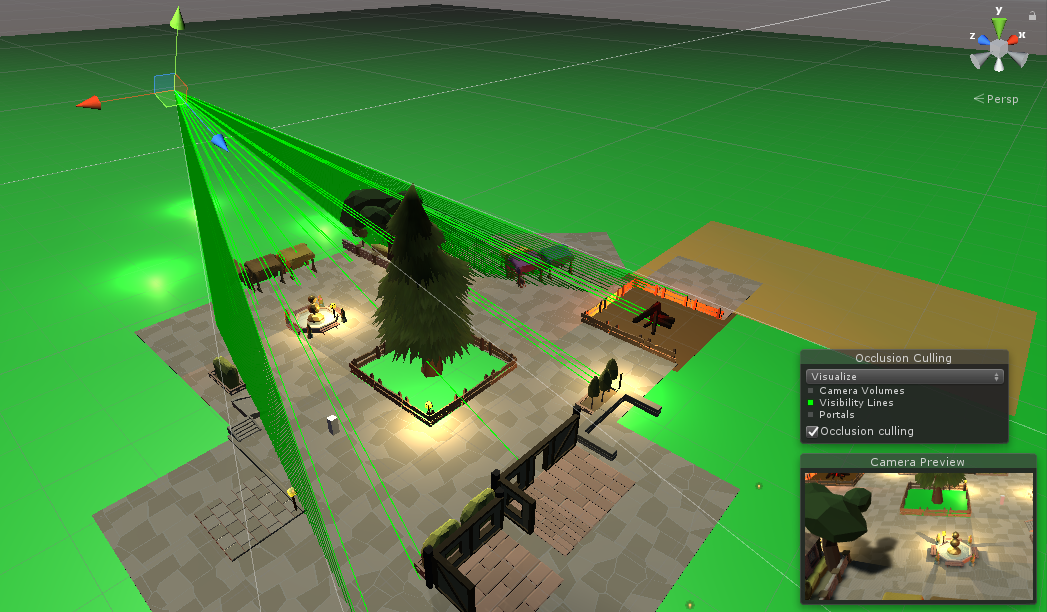
\includegraphics[scale=0.475]{images/village/occlusion_culling.PNG}
\caption{Occlusion Culling, Ignorieren von Objekten außerhalb des Sichtfeldes}
\label{fig:occlusion_culling}
\end{figure}

Unity stellt weiterhin eine Visualisierung für das Verfahren zur Verfügung. In der Abbildung \ref{fig:occlusion_culling} ist ein Beispiel für Occlusion Culling zu sehen. Das ausgewählte Objekt, das an den drei Achsen erkannt werden kann, ist die aktive Kamera der Szene. Ihre Position, Ausrichtung und die Breite ihres Sichtfelds bestimmen, welche Objekte berechnet werden müssen. In der rechten unteren Ecke der Abbildung ist der Ausschnitt der Szene zu erkennen, der von der Kamera wahrgenommen wird. In der Szene kann einfach erkannt werden, dass alle weiteren Objekte des Dorfes nicht angezeigt werden, weil sie vom Blickwinkel der Kamera nicht erfasst werden.
Die folgende Grafik \ref{fig:occlusion_culling_2} zeigt weiterhin, wie Objekte durch andere Objekte verdeckt werden. Hinter dem großen Gebäude im Vordergrund werden keine Objekte berechnet, das sie durch das Haus verdeckt werden. 

\begin{figure}[H]
\centering
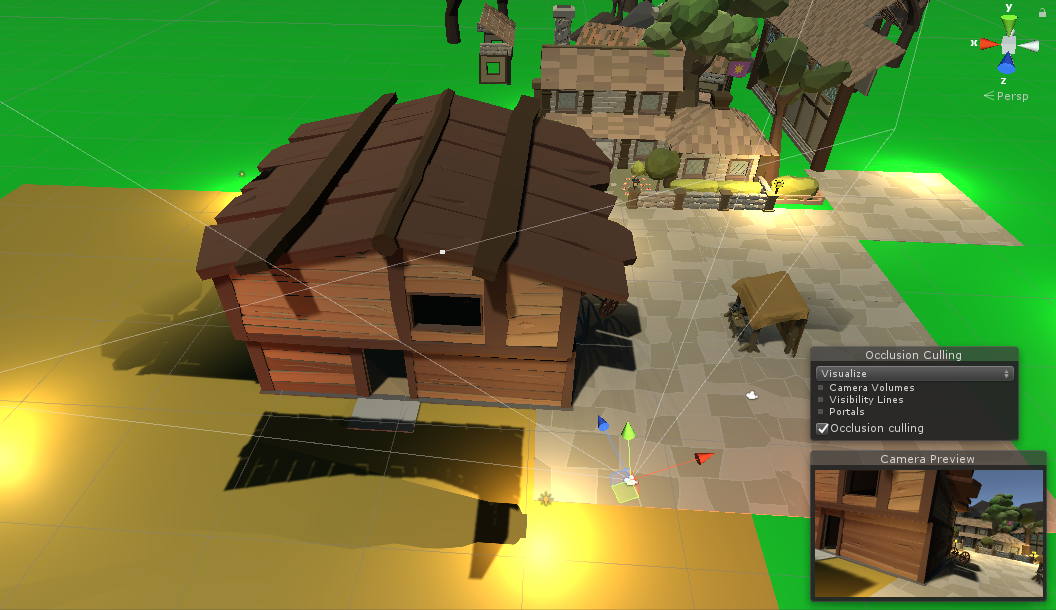
\includegraphics[scale=0.475]{images/village/occlusion_culling_2.PNG}
\caption{Occlusion Culling, Ignorieren von Objekten durch Verdeckung}
\label{fig:occlusion_culling_2}
\end{figure}



% anfangs wurden berufe nicht fest zugewiesen. bei der entscheidungsfindung konnten agenten aus allen work-aktionen auswählen, basierend auch auf der menge der resourcen. das hat dazu geführt, dass viele npcs das gleiche tun. daher wurden jobs fest zugewiesen. damit dann trotzdem die richtige menge von ressourcen produziert wurde, wurde der villageagent eingeführt. aber der funktioniert halt leider nicht.


\section{Verschiedene Ansätze für Ressourcensystem und VillageAgent}
Wie bereits in den Abschnitten \ref{village_village_agent} und \ref{gameacademy} beschrieben, sind durch die Parameter der \inlinecode{GameAcademy} verschiedene Ansätze für die Behandlung von Ressourcen und Berufen in der Simulation auswählbar. Insgesamt ergeben sich drei Möglichkeiten für die Verwaltung von Ressourcen:

\begin{itemize}
    \item \textit{Ansatz 1}: Keine Zuweisung von Berufen für Agenten. Es werden keine Berufsaktionen maskiert, stattdessen können Agenten die Aktionen frei wählen. Die Ressourcen werden durch die Auswahl der Aktionen der Agenten indirekt in der Balance gehalten.
    \item \textit{Ansatz 2}: Nutzung fest zugewiesener Berufe für Agenten sowie Maskierung aller Aktionen, die nicht zum Beruf gehören. Kontinuierliche Anpassung der Berufe durch den \inlinecode{VillageAgent} zur indirekten Verwaltung der Ressourcen.
    \item \textit{Ansatz 3}: Nutzung fest zugewiesener Berufe für Agenten ohne eine Anpassung durch den \inlinecode{VillageAgent}. Statt eine Lösung für das Ressourcenproblem zu finden, werden Ressourcen vollständig ignoriert und sind für die Entscheidungsfindung nicht mehr relevant.
\end{itemize}

Die Verwendung eines Ressourcensystems führt dazu, dass die Agenten lernen müssen, mit diesen Ressourcen umzugehen. Es besteht das Risiko, dass die Ressourcen des Dorfsystems ab einem gewissen Punkt nicht mehr in der Balance gehalten werden. Vor dem Training ist nicht absehbar, wie viele Ressourcen von den Agenten verbraucht werden, da nicht klar ist, welche Entscheidungen diese treffen. Es ist daher schwierig, für die Aktionen der Agenten sinnvolle Parameter bezüglich der Kosten und Erlöse von Ressourcen festzulegen. Daher werden Tests durchgeführt, die bestimmen sollen, mit welcher der drei oben genannten Verfahren das Problem am besten gelöst werden kann. Dazu gehört auch unter Umständen die Maßnahme, auf die Nutzung von Ressourcen gänzlich zu verzichten (Ansatz 3), falls kein zufriedenstellendes Ergebnis erzielt werden kann. 

Bevor weitere Aspekte des Trainings betrachtet werden, wird zunächst ein Vergleich zwischen drei Testtrainingsvorgängen der drei vorgeschlagenen Ansätze aufgestellt. In der Abbildung \ref{fig:diagram_test_resource_run_1} werden die Trainigsverläufe dargestellt.

\begin{figure}[H]
\centering
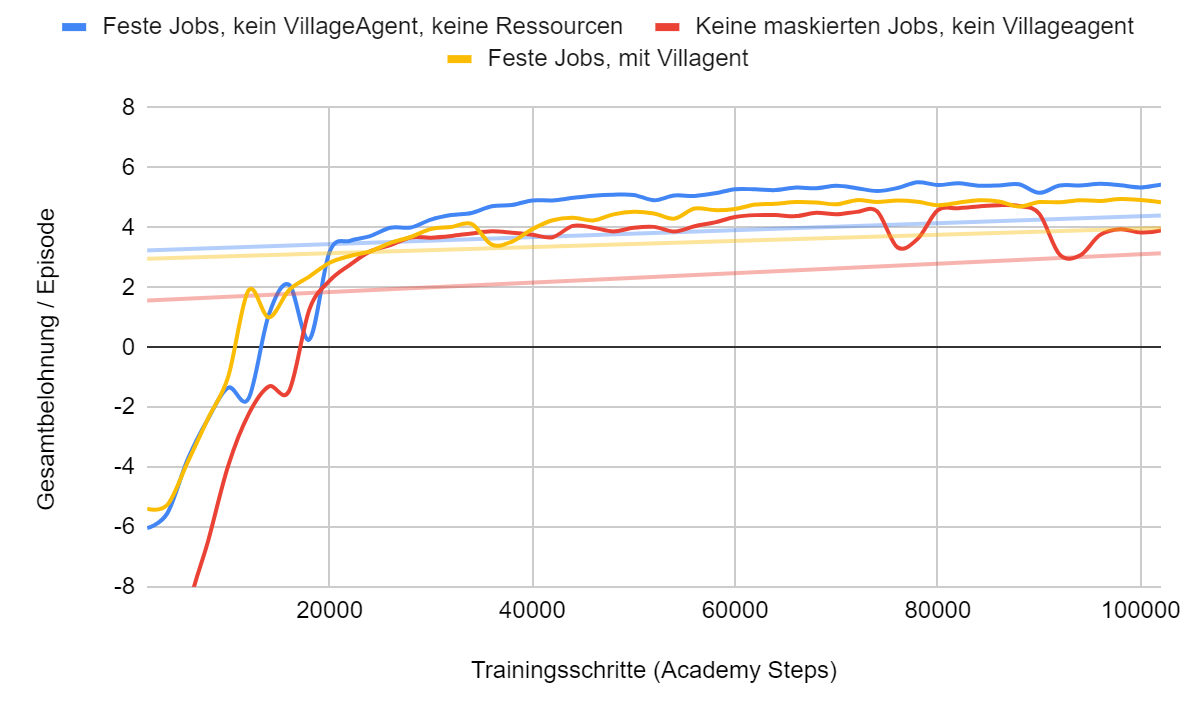
\includegraphics[scale=0.475]{images/training/diagram_test_resource_run_1.png}
\caption{Trainingsverläufe für \inlinecode{NpcAgent}s, verschiedene Ansätze für das Ressourcensystem}
\label{fig:diagram_test_resource_run_1}
\end{figure}

Grundsätzlich haben sich für alle Ansätze ähnliche Verläufe ergeben. Anhand der eingezeichneten Trendlinien kann man erkennen, dass sich für den ersten Ansatz insgesamt die niedrigsten akkumulierten Belohnungen ergeben haben. Das kann dadurch erklärt werden, dass ein insgesamt größerer Aktionsraum verwendet wurde. Dadurch wird das Training erschwert, weil dieser größere Aktionsraum erforscht werden muss, um Assoziationen zwischen Aktionen und Beobachtungen herzustellen. Für den zweiten Ansatz ergibt sich eine nur geringfügig niedrigere Belohnung im Vergleich zum ersten Ansatz. Aktionen werden im zweiten Ansatz öfter maskiert, weil Ressourcen nicht zur Verfügung stehen. Das kann dazu führen, dass Agenten gewünschte Aktionen nicht ausführen können, weil zu wenig Ressourcen vorhanden sind. Da diese Limitierungen für den dritten Ansatz nicht gelten und der Aktionsraum kleiner ist, wurden dort die höchsten Belohnungen erreicht. Nur im zweiten Ansatz wurde der \Fachbegriff{VillageAgent} verwendet. Neben den \inlinecode{NpcAgent}s mussten im entsprechenden Trainingsvorgang also auch \inlinecode{VillageAgent}s trainiert werden.
Insgesamt konvergieren alle drei Ansätze bereits nach etwa 400.000 Trainingsschritten. Die Graphen beschreiben anschließend einen nahezu flachen Verlauf. Ein signifikanter Lernvorgang ist nach dem Erreichen dieses Punktes nicht mehr zu erwarten.  

\begin{figure}[H]
\centering
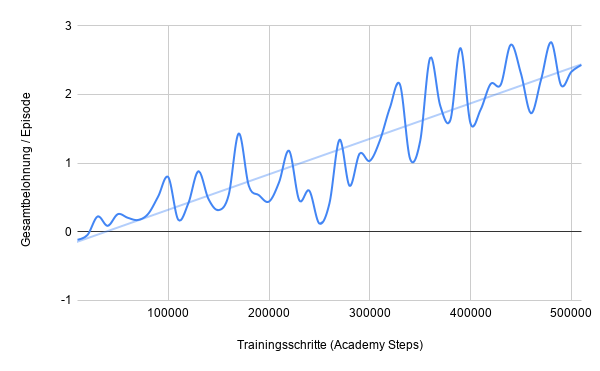
\includegraphics[scale=0.7]{images/training/diagram_test_resource_run_villageagent.png}
\caption{Trainingsverlauf des \inlinecode{VillageAgent}}
\label{fig:diagram_test_resource_run_villageagent}
\end{figure}

 In Abbildung \ref{fig:diagram_test_resource_run_villageagent} ist der Trainingsverlauf des \inlinecode{VillageAgent} zu erkennen. Der Verlauf der akkumulierten Belohnung steigt nicht monoton an. Es bildet sich ein eher unstabiles Training mit vielen lokalen Maxima und Minima ab. An der Trendlinie ist jedoch klar erkennbar, dass insgesamt ein Lernvorgang durch ein Wachstum der Belohnungen stattfindet. Weiterhin wird durch den Graphen bis zum Ende des Trainingsvorgangs kein Plateau abgebildet. Die akkumulierten Belohnungen verändern sich kontinuierlich. Aus diesem Grund wird ein erweiterter Trainingsprozess für den \inlinecode{VillageAgent} mit einer höheren Anzahl von Trainingsschritten durchgeführt, wie in Abbildung \ref{fig:diagram_test_resource_run_villageagent_LARGE} zu sehen.
 
\begin{figure}[H]
\centering
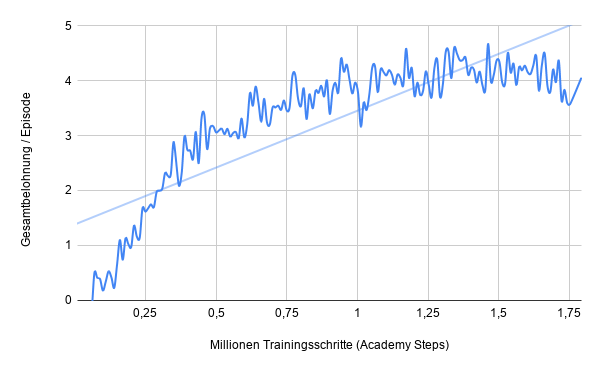
\includegraphics[scale=0.7]{images/training/diagram_test_resource_run_villageagent_LARGE.png}
\caption{Erweiterter Trainingsverlauf des \inlinecode{VillageAgent}}
\label{fig:diagram_test_resource_run_villageagent_LARGE}
\end{figure}

Auch im erweiterten Trainingsprozess ist zu erkennen, dass der entsprechende Graph nicht monoton steigt, sondern starke Schwankungen aufweist. Trotzdem ist wie bereits oben beschrieben ein konstantes Wachstum zu verzeichnen. Zum Ende des Verlaufs ist zu erkennen, dass der Graph einen flachen Verlauf beschreibt und das Wachstum der Belohnungen zum Stillstand kommt. Nach knapp mehr als einer Million Schritten wird annähernd ein Plateau erreicht.





% experimentiert mit resource rewards?


% rewards wurden erklärt, jetzt das wa seigentlich schief gelaufen ist (agenten sind dumm, oszillierender villageagent)







% beschreiben wie die trainingsverläufe aussehen


Die Betrachtung der akkumulierten Belohnungen alleine reicht allerdings noch nicht aus, um das Verhalten der Agenten zu beurteilen. Die aus den Trainingsvorgängen enstandenen Modelle bzw. Policies wurden daher im Inference-Modus der Simulation verwendet, um das Verhalten der Agenten zu betrachten und dadurch die Auswahl der verwendeten Ansätze zu beeinflussen. Es wurden jeweils mehrere Spielzeittage betrachtet, um das resultierende Verhalten der Agenten zu analysieren.

Im ersten Ansatz war auffällig, dass häufig viele Agenten den selben Beruf gewählt haben. Zeitweise haben etwa die Hälfte der 50 pro Dorf verwendeten Agenten dieselbe berufliche Tätigkeit ausgeführt. Die Agenten haben also nicht gelernt, Berufsaktionen aufgrund der aktuell vorhandenen Ressourcen zu wählen. Das führte dazu, dass das Ressourcensystem nicht in der Balance gehalten wurde und Defizite für bestimmte Ressourcen entstanden. Aus diesem Grund konnten nach einiger Zeit bestimmte Aktionen nicht mehr ausgeführt werden, weil ihre ressourcenbasierten Bedingungen nicht erfüllt wurden. Die trotzdem hohe Belohnung der Agenten ist darauf zurückzuführen, dass für maskierte Aktionen aufgrund von fehlenden Ressourcen in der Regel Alternativen verfügbar sind. Wenn zum Beispiel kein Bier mehr vorhanden ist, kann zwar die Freizeitaktion \Fachbegriff{Taverne} nicht mehr ausgeführt werden, wohl aber die Freizeitaktion \Fachbegriff{Visit}. Die Vielfältigkeit der Aktionen der Agenten wird dadurch jedoch eingeschränkt. Weiterhin bringt etwa das Ausführen der Berufsaktion \inlinecode{Logging} bei einem gegebenen Arbeitsbedürfnis die gleiche Belohnung wie die Aktion \inlinecode{Hunting}, sodass kein direkter Anreiz in Form von Belohnungen geboten wird, um unterschiedliche Berufsaktionen auszuführen. Die Verwendung der Ressourcen als Observations reicht daher nicht aus, um die Wahl der Beufsaktionen maßgeblich zu beeinflussen.
Verschiedene Ideen wurden verfolgt, um dieses Problem einzudämmen. Beispielsweise wurde für jede ausgeführte Aktion des Agenten eine zusätzliche Belohnung bzw. Bestrafung verteilt, die auf die Menge der Ressourcen zurückgeführt wurde - unabhängig davon, welche Aktion ausgeführt wurde. Außerdem wurde der Versuch unternommen, die Belohnungen beruflicher Aktionen an den produzierten Ressourcen im Vergleich zur aktuellen Menge der entsprechenden Ressource zu messen. Eine hohe Belohnung wurde dann erzielt, wenn ein Job ausgeführt wurde, dessen mit ihm verbundene Ressource nicht ausreichend vorhanden war.
Diese unternommenen Versuche konnten das Problem jedoch nicht beheben bzw. verschlechterten dieses teilweise. 

Daher wurde der im zweiten Ansatz verwendete \Fachbegriff{VillageAgent} entwickelt, der die Menge Ressourcen auf einem stabilen Level halten soll. Weiterhin wurden dafür die festen Berufe bzw. \Fachbegriff{Jobs} für Agenten eingeführt, die dazu führen, dass alle Aktionen eines Agenten, die nicht mit seinem Job assoziiert sind, maskiert werden. Für den Inference-Modus wurde der zweite, erweiterte Trainingsverlauf des \inlinecode{VillageAgent} verwendet (siehe Abbildung \ref{fig:diagram_test_resource_run_villageagent_LARGE}), um die bestmögliche Policy zu nutzen.
Wie bereits in Abschnitt \ref{village_village_agent} angedeutet, fällen alle verwendeten Agenten vom Typ \inlinecode{VillageAgent} immer dann eine Entscheidung, wenn ein Zähler in der \inlinecode{GameAcademy} einen bestimmten Wert erreicht. Die laufende Episode wird abgebrochen, sobald eine bestimmte Anzahl von Entscheidungen getroffen wurde. Der Zähler wird jedes mal inkrementiert, wenn ein \inlinecode{NpcAgent} eine Aktion ausführt. Die entsprechenden Parameter in der \inlinecode{GameAcademy} wurden so gewählt, dass alle \inlinecode{VillageAgent}s Entscheidungen ausführen, sobald jeder \inlinecode{NpcAgent} fünf Aktionen ausgeführt hat. Insgesamt sind zehn dieser Entscheidungen notwendig, um die Episode abzuschließen. Mit sechs verwendeten Dörfer und 50 pro Dorf verwendeten Agenten werden daher 1500 NPC-Aktionen gebraucht, um eine Entscheidung auszulösen und 15.000, um die Episode zu beenden.
Der \inlinecode{VillageAgent} erhält Belohnungen, wenn richtige Entscheidungen getroffen werden und Bestrafungen, wenn kontraproduktive Entscheidungen getroffen werden. Trotz eines kontinuierlichen Lernvorgangs und einer deutlich positiven akkumulierten Gesamtbelohnung kommt es nicht dazu, dass das Ressourcensystem durch eine Anpassung der Berufe in Waage gehalten wird. Das System oszilliert stark und lernt nicht ausreichend, Entscheidungen zu treffen, die auf der aktuellen Menge der Ressourcen beruhen. Ein grundlegendes Problem bei diesem Vorgang ist die Häufigkeit der Entscheidungen, die durch den Agenten gefällt werden - auf 1000 gesammelte Erfahrungen durch \inlinecode{NpcAgent}s kommen lediglich ca. 4 Erfahrungen des \inlinecode{VillageAgent}s. Der \inlinecode{VillageAgent} muss also aus einer Menge von Entscheidungen eine Policy erlernen, die nur einem Anteil von 0.4\% der entsprechenden Menge des \inlinecode{NpcAgent} entspricht. Um den Zustandsraum des Agenten hinreichend zu erkunden, muss vermutlich eine deutlich höhere Anzahl von Erfahrungen gesammelt werden. Ein zusätzliches potentielles Problem besteht darin, dass die Auswirkungen der Entscheidungen auf die tatsächlichen Ressourcenmengen eine starke zeitliche Verzögerung haben, da Agenten nur etwa ein mal am Tag arbeiten. Das kann theoretisch dazu führen, dass die gleichen Aktionen mehrfach ausgeführt werden, weil die Menge der Ressourcen sich seit der letzten Entscheidung nicht signifikant verändert hat. Es wurden Versuche unternommen, diese Probleme zu lösen, indem die Belohnungen und die Intervalle der \inlinecode{VillageAgent}-Entscheidungen angepasst wurden. Diese Versuche führten ebenfalls dazu, dass den NPCs falsche Berufe zugewiesen wurden.

Aus diesem Grund wird der dritte Ansatz verwendet, in dem das Ressourcensystem ignoriert wird. Aktionen produzieren und verbrauchen dann keinerlei Ressourcen mehr. Weiterhin werden keine ressourcenbasierte Observations getätigt und keine Belohnungen an Ressourcen gebunden.

Dadurch wird der Simulation ein kleiner Teil ihrer Komplexität genommen. Die Glaubwürdigkeit der Entscheidungsfindung der NPCs wird dadurch allerdings nicht beeinflusst, da diese maßgeblich von den Bedürfnissen des Agenten abhängt. Die Nutzung von Ressourcen fungiert viel mehr als limitierender Faktor. Um die Agenten tatsächlich authentischer wirken zu lassen, müsste das Ressourcensystem um Faktoren wie Handel zwischen verschiedenen Dörfern erweitert werden. Da dies nicht gegeben ist, stellt das Ignorieren des Ressourcensystems keine Verschlechterung dar.    




\section{Wahl der initialen Hyperparameter}\label{village_training_hyperparameter}
Die Tabelle \ref{tab:ml-agents_training_hyperparameters} zeigt eine Übersicht über die wichtigsten Hyperparameter für das Training der Agenten. Diese werden in einer Konfigurationsdatei definiert, wie in Abschnitt  \ref{ml_unity} beschrieben. Für die Erstellung der Übersicht dient eine Tabelle aus der ML-Agents Dokumentation als Grundlage \cite{ml-agents_documentation_hyperparameter_ppo}, die Empfehlungen für die Parameter ausspricht. Alle nicht \ac{ppo}-basierten Parameter wurden aus der Tabelle entfernt, da sie für diese Arbeit nicht weiter relevant sind.

\smallskip
\begin{table}[H]
\begin{tabular} {|  p{3.2cm}  |  p{12.4cm}  |} \hline
\textbf{Setting} & \textbf{Description} \\ \hline
batch\_size & The number of experiences in each iteration of gradient descent. \\ \hline
beta & The strength of entropy regularization. \\ \hline
buffer\_size & The number of experiences to collect before updating the policy model. \\ \hline
epsilon & Influences how rapidly the policy can evolve during training. \\ \hline
hidden\_units & The number of units in the hidden layers of the neural network. \\ \hline
lambd & The regularization parameter. \\ \hline
learning\_rate & The initial learning rate for gradient descent. \\ \hline
max\_steps & The maximum number of simulation steps to run during a training session. \\ \hline
memory\_size & The size of the memory an agent while training with a recurrent network. \\ \hline
normalize & Whether to automatically normalize observations. \\ \hline
num\_epoch & The number of passes to make through the experience buffer when performing gradient descent optimization. \\ \hline
num\_layers & The number of hidden layers in the neural network. \\ \hline
behavioral\_cloning & Use demonstrations to bootstrap the policy neural network. \\ \hline
reward\_signals & The reward signals used to train the policy. Curiosity and GAIL can be enabled here. Gamma can also be set here. \\ \hline
sequence\_length & Defines how long the sequences of experiences must be while training. Only used for training with a recurrent neural network. \\ \hline
summary\_freq & How often, in steps, to save training statistics. This determines the number of data points shown by TensorBoard. \\ \hline
time\_horizon & The amount of experiences collected per-agent before adding it to the experience buffer. \\ \hline
use\_recurrent & Train using a recurrent neural network. \\ \hline
\end{tabular}
\caption{ML-Agents-Hyperparameter für das Training \cite{ml-agents_documentation}}
\label{tab:ml-agents_training_hyperparameters}
\end{table}

Ein Großteil dieser Parameter wurde bereits durch mathematische Grundlagen im Kapitel \ref{reinforcement_learning}  definiert. Die Funktion weiterer Parameter geht entweder aus der Beschreibung innerhalb der Tabelle hervor oder wird in der folgenden Tabelle \ref{village_training_hyperparameter} erläutert. Einige der Parameter sind optional.


Für das Training der Agenten wurden mehrere Trainingsvorgänge mit unterschiedlichen Hyperparametern durchgeführt, die später miteinander verglichen werden. Als Grundlage für das Training wird der im vorherigen Abschnitt beschriebene Trainingsvorgang für den dritten Ansatz der Lösung für den Umgang mit Ressourcen verwendet. Die in diesem Vorgang verwendete Trainingskonfiguration, die im Folgenden vorgestellt wird, stellt eine Basiskonfiguration dar, die das Fundament für weitere Trainingsvorgänge bildet. In diesen Vorgängen werden jeweils einzelne Parameter aus der Konfiguration angepasst. Dadurch sollen möglichst ideale Hyperparameter identifiziert werden. Bereits die in der Basiskonfiguration festgelegten Parameter wurden empirisch ermittelt, indem während der Entwicklung des Dorfes zahlreiche Trainingsvorgänge durchgeführt wurden.
Schließlich wird ein finales Training durchgeführt, das die besten verwendeten Hyperparameter nutzt und so ein optimales Ergebnis erzielen soll. Im Folgenden werden Hyperparameter für den zugrunde liegenden Trainingsvorgang beschrieben. Für die initiale Festlegung der Trainingsparameter wurden teilweise Empfehlungen aus der Dokumentation des ML-Agents Frameworks hinzugezogen \cite{ml-agents_documentation_hyperparameter_ppo}. Ein Großteil der Parameter wurde bereits im Kapitel \ref{reinforcement_learning} erläutert und ist auf die mathematischen Grundlagen des Verfahrens zurückzuführen. Folgende Parameter wurden für das Basistraining verwendet:

\smallskip
\begin{table}[H]
\footnotesize
\centering
\begin{tabular} {|  p{3.5cm}  |  p{3cm}  |} \hline
\textbf{Parameter} & \textbf{Beschreibung} \\ \hline

\Fachbegriff{trainer}  &  ppo  \\ \hline
\Fachbegriff{epsilon}  &  0.2  \\ \hline
\Fachbegriff{lambd}  &  0.925  \\ \hline
\Fachbegriff{learning\_rate\_schedule}  &  linear  \\ \hline
\Fachbegriff{learning\_rate}  &  4e-4  \\ \hline
\Fachbegriff{max\_steps}  &  5e5  \\ \hline
\Fachbegriff{normalize}  &  false  \\ \hline
\Fachbegriff{batch\_size}  &  32  \\ \hline
\Fachbegriff{buffer\_size}  &  8192  \\ \hline
\Fachbegriff{num\_epoch}  &  4  \\ \hline
\Fachbegriff{time\_horizon}  &  512  \\ \hline
\Fachbegriff{beta}  &  1.2e-2  \\ \hline
\Fachbegriff{summary\_freq}  &  2000  \\ \hline
\Fachbegriff{num\_layers}  &  3  \\ \hline
\Fachbegriff{hidden\_units}  &  256  \\ \hline
\Fachbegriff{use\_recurrent}  &  false  \\ \hline
\Fachbegriff{memory\_size}  &  128  \\ \hline
\Fachbegriff{sequence\_length}  &  128  \\ \hline
\Fachbegriff{reward\_signals}  &  extrinsic  \\ \hline
\Fachbegriff{reward\_strength}  &  1.0  \\ \hline
\Fachbegriff{gamma}  &  0.93  \\ \hline

\end{tabular}
\caption{Gewählte Hyperparameter für das Basistraining.}
\label{tab:base_training_hyperparameters}
\end{table}

Als zugrunde liegender Algorithmus wird \ac{ppo} verwendet. \Fachbegriff{epsilon} wird auf $ 0.2 $ festgelegt. Der Wert bestimmt, wie groß Änderungen der Policy minimal sein müssen. Über den Parameter \Fachbegriff{lambd} kann definiert werden, wie sehr sich der Algorithmus auf die Vorhersage (bzw. \Fachbegriff{Value Estimate}) der Belohnung im Gegensatz zur eigentlichen erfahrenen Belohnung einer Aktion verlässt. Es wird eine Lernrate mit dem Wert $4 * 10^{-4}$ verwendet, die sich im Verlauf des Trainingsvorgangs linear bis zum Wert $0$ beim letzten Trainingsschritt verringert. Insgesamt werden dafür 500.000 Trainingsschritte verwendet. Eine Normalisierung der Observations findet nicht statt, da alle Beobachtungen manuell normalisiert werden.
Weiterhin muss ein Wert für die \Fachbegriff{buffer\_size} festgelegt werden. Dadurch wird beschrieben, wie viele Entscheidungen gesammelt werden sollen, bevor ein Update der Policy stattfindet. Dieser Buffer wird in Batches von der Größe \Fachbegriff{batch\_size} aufgeteilt. Für jeden dieser Batches wird ein Gradientenverfahren durchgeführt, um das neue, angepasste Modell zu berechnen. Der Parameter \Fachbegriff{num\_epoch} legt fest, wie oft dieser Prozess wiederholt werden soll. Der Parameter \Fachbegriff{time\_horizon} legt fest, wie viele Entscheidungen auf einmal in den Buffer geschrieben werden sollen. Wenn die Kapazität des Buffers vor dem Beenden einer Episode erreicht wurde, wird ein \Fachbegriff{Value Estimate} gebildet, um die zukünftigen Belohnungen des Agenten der Episode zu schätzen. \Fachbegriff{buffer\_size} und \Fachbegriff{time\_horizon} müssen daher logischerweise ein Vielfaches der \Fachbegriff{batch\_size} sein. Diese Parameter wurden durch Empfehlungen des Frameworks und empirische Beobachtungen ausgewählt. Konkret wurden noch während der Entwicklung der Dorfsimulation verschiedene Trainingsvorgänge ausgeführt, wobei sich bestimmte Parameter bewährt haben.

Über den Wert \Fachbegriff{beta} wird definiert, wie zufällig die Aktionen der Agenten ausgewählt werden, um zu gewährleisten, dass der Aktionsraum des Agenten sinnvoll erkundet wird. Damit wird also direkt die Entropie beeinflusst, die festlegt, wie zufällig die Entscheidungen eines Brains sind. Der Wert sollte so ausgewählt werden, dass die Entropie des Trainingsvorgangs stetig sinkt.

Über die \Fachbegriff{summary\_freq} kann die Schrittgröße für die Ausgabe der durchschnittlichen akkumulierten Belohnung der Agenten in der Konsole bestimmt werden. Größere Werte führen zu einem zu hohen Intervall zwischen Statusberichten. Zu kleine Werte führen zu einer starken Varianz bezüglich der erfahrenen Belohnungswerte. In diesem Fall wird für jeweils 2.000 durchgeführte Trainingsschritte ein Statusbericht angegeben. 

Die Parameter \Fachbegriff{num\_layers} und \Fachbegriff{hidden\_units} sind essentiell für den Aufbau des neuronalen Netzes. Insgesamt werden drei Schichten mit je 512 enthaltenen Neuronen verwendet. Es wird kein rekurrentes neuronales Netz verwendet, da der Parameter \Fachbegriff{use\_recurrent} auf \Fachbegriff{false} gesetzt wird. Die \Fachbegriff{memory\_size} bestimmt die Größe für einzelne \sogenannt{Erinnerungen} für die Rückkopplungen in dem rekurrenten Netz. Über den Parameter \Fachbegriff{sequence\_length} wird zudem festgelegt, wie viele dieser Erinnerungen verwendet werden sollen. Diese Parameter werden nur für rekurrente neuronale Netze verwendet und sind daher zunächst nicht relevant.

Der Wert des \Fachbegriff{reward\_signals} bestimmt, welche Art von Belohnungen das Verfahren verwendet und wird daher auf \Fachbegriff{extrinsic} festgelegt. Damit sind die Belohnungen gemeint, die in der Simulation festgelegt wurden. Es können zusätzliche \Fachbegriff{reward\_signals} festgelegt werden, um mehrere Belohnungsarten zu nutzen. Durch \Fachbegriff{curiosity}-Belohnungen erhält der Agent immer dann Belohnungen, wenn er von seiner Policy abweicht, um den Aktionsraum zu erkunden. Das ist dann sinnvoll, wenn extrinsische Belohnungen sehr selten sind und nur durch \sogenannt{Ausprobieren} gefunden werden können. Da in diesem Fall jede Aktion eine Belohnung zur Folge hat, werden zunächst keine derartigen Belohnungen verwendet. Zusätzlich können \Fachbegriff{GAIL}-Belohnungen verwendet werden, die nicht relevant sind, da sie bei Imitation Learning zum Einsatz kommen.
Konkret werden extrinsische Belohnungen mit einem Multiplikator \Fachbegriff{reward\_strength} von $1.0$ verwendet, da die in der Simulation definierten Belohnungen nicht verändert werden sollen. Weiterhin wird ein relativ niedriger Wert \Fachbegriff{gamma} festgelegt. Dieser Parameter beschreibt den in Kapitel \ref{reinforcement_learning} definierten Wert $ \gamma $ und bestimmt, wie sehr zukünftige Belohnungen Entscheidungen des Agenten beeinflussen. 
Für $ \gamma\ $ wird ein niedriger Wert gewählt, sodass zukünftige Zustände des Agenten weniger relevant sind. Es wird davon ausgegangen, dass für die Befriedigung von menschlichen Bedürfnissen hauptsächlich der aktuelle Zustand relevant ist. 



\section{Güteüberprüfung}
Beim überwachten Lernen werden häufig direkte Bewertungskriterien genutzt, indem Werte für \Fachbegriff{Precision}, \Fachbegriff{Recall} oder \Fachbegriff{F1} gebildet werden. Da beim \ac{reinforcement_learning} keine Klassifizerung stattfindet und keine gelabelten Daten vorhanden sind, ist ein derartiges Vorgehen hier nicht möglich. Ein exakter Wert für die Genauigkeit der Ergebnisse kann daher nicht gebildet werden.
Um die Güte der Trainingsergebnisse zu überprüfen, können alternative Metriken verwendet werden. Neben der Höhe der Belohnungen wird die \Fachbegriff{Value Loss}-Funktion verwendet. Sie beschreibt die Verlustfunktion (siehe Abschnitt \ref{loss_functions}) bezüglich der Value Function des Agenten und gibt damit an, wie gut das Modell Belohnungen zukünftiger Zustände vorhersagen kann. Weiterhin wird der  Entropieverlauf genutzt, der die Zufälligkeit der gewählten Aktionen bestimmt. Die Daten können im Tensorboard betrachtet und von dort exportiert werden. Im Normalfall kann man auch an der Länge der Episoden den Lernvorgang bewerten. Die Länge der Episoden der Agenten ist hier aber nicht relevant, da die Episoden stets nach einer festgelegten Anzahl von Aktionen enden.

Mit den genannten Metriken kann zwar der Erfolg des Trainingsvorgang aus einer mathematischen Sicht evaluiert werden, sie bieten jedoch nur Hinweise darüber, wie authentisch das resultierende Verhalten der Agenten ist. Um das tatsächliche Verhalten zu bewerten, reichen diese Metriken also nicht aus. Hohe Belohnungen könnten zum Beispiel auch entstehen, wenn ein Agent lernt, einen Fehler in der Simulation auszunutzen. Daher müssen die Agenten konkret innerhalb der Simulation im Inference-Modus beobachtet werden. Dafür können die entwickelten UI-Elemente, die Auskunft über verschiedene Informationen des Dorfes wie der Anzahl der aktuell ausgeführten Aktionen bieten, genutzt werden. Diese Informationen bieten einen schnellen Überblick über das erlernte Verhalten der Agenten. Im Abschnitt \ref{7_result_agent_behavior} wird neben Metriken wie der Entropie oder den Belohnungen der Agenten daher zusätzlich das Verhalten der Agenten betrachtet.













\section{Trainingsergebnisse}
Wie im vorherigen Abschnitt erwähnt, wurde eine Basiskonfiguration für Trainingsvorgänge erstellt, auf deren Grundlage Trainingsvorgänge durchgeführt werden. Einzelne Parameter werden für diese Vorgänge angepasst, anschließend wird ein Vergleich der Ergebnisse durchgeführt.

Zunächst wird der Basistrainingsvorgang näher betrachtet.

\subsection{Basistraining}
In den Abbildungen \ref{fig:diagram_test_resource_run_entropy}, \ref{fig:base_value-loss} und \ref{fig:base_reward} sind Informationen zum Basistrainingsverlauf zu erkennen. Auf den horizontalen Achsen der Diagramme ist jeweils die Anzahl der Trainingsschritte eingezeichnet.

\begin{figure}[H]
\centering
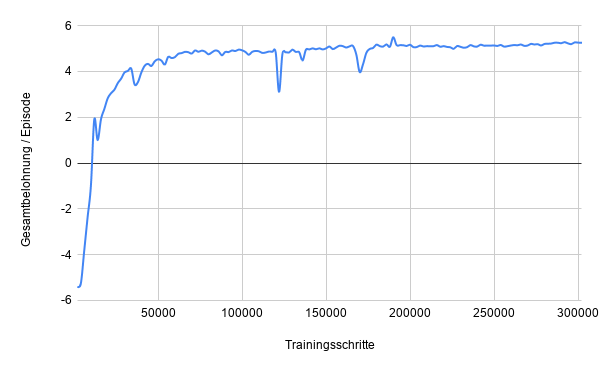
\includegraphics[scale=0.7]{images/training/base_reward.png}
\caption{Akkumulierte Belohnungen im Basistraining des \inlinecode{NpcAgent}}
\label{fig:base_reward}
\end{figure}

\begin{figure}[H]
\centering
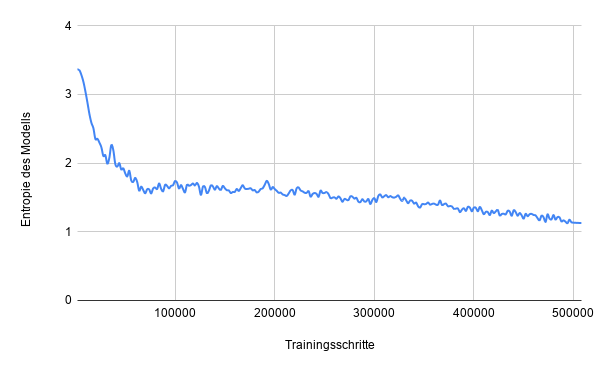
\includegraphics[scale=0.7]{images/training/base_value-loss.png}
\caption{Value Loss im Basistraining des \inlinecode{NpcAgent}}
\label{fig:base_value-loss}
\end{figure}

Die Abbildung \ref{fig:base_value-loss} zeigt den Verlauf des \Fachbegriff{Value Loss}, also die Verlustfunktion bezüglich der Value Function. Solange der Graph einen absteigenden Verlauf beschreibt, lernt der Agent, die Value Function zu optimieren.

\begin{figure}[H]
\centering
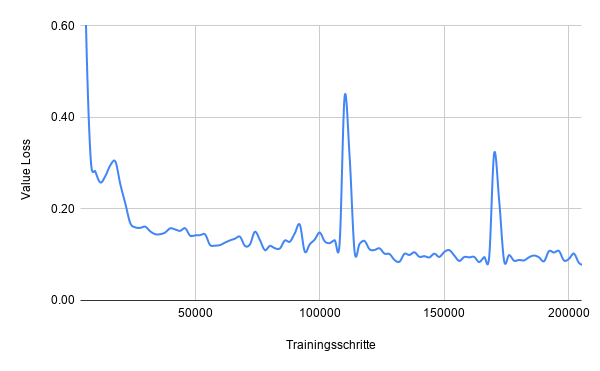
\includegraphics[scale=0.7]{images/training/base_entropy.png}
\caption{Entropieverlauf im Basistraining des \inlinecode{NpcAgent}}
\label{fig:diagram_test_resource_run_entropy}
\end{figure}

Die Entropie wurde auf den Wert $ 1.2 * 10^{-2}$ festgelegt. Daraus ergibt sich der in Abbildung \ref{fig:diagram_test_resource_run_entropy} sichtbare Entropieverlauf. Die stetige Verringerung der Entropie mit einer steigenden Anzahl der Trainingsschritte belegt, dass ein guter Wert gewählt wurde.

Weiterhin beschreibt die Abbildung \ref{fig:base_reward} die akkumulierten Belohnungen für das Basistraining, wie bereits in Teilen in Abbildung \ref{fig:diagram_test_resource_run_1} zu sehen. Man kann erkennen, dass sich die Spitzen der Belohnungsfunktion bei etwa  125.000 und 170.000 Zeitschritten im Value Loss-Diagramm widerspiegeln. Typischerweise sinkt die Verlustfunktion so lange, wie die Belohnung des Agenten zunimmt. Weiterhin sind keine Auffälligkeiten zu erkennen.










\subsection{Optimierung der Ergebnisse durch Anpassung der Hyperparameter}
Um optimale Parameter zu definieren, wurde eine Reihe von Trainingsvorgängen durchgeführt. In jedem dieser Durchläufe wurde ein einzelner Parameter aus der Basiskonfiguration angepasst, um die Auswirkungen der Änderung isoliert zu betrachten. Das Ergebnis wird mit anderen Trainingsvorgängen verglichen, in dem der selbe Parameter verändert wurde. Es wird geprüft, ob die Veränderung eine Verbesserung erzielt. Der Parameter mit dem besten Trainingsresultat wird anschließend für ein finales Training gewählt und in die finale Konfigurationsdatei eingetragen. Über mehrere Tage wurden dafür Trainingsdurchläufe durchgeführt. 
Die jeweilige Dauer der durchgeführten Trainingsvorgänge kann in der Abbildung \ref{fig:training_durations} betrachtet werden. Auffällig ist, dass das Training mit einem rekurrenten Netzwerk deutlich mehr Zeit beansprucht, da durch die zusätzlichen Verbindungen der Neuronen im Netzwerk ein höherer Rechenaufwand entsteht. Darüber hinaus sind keine Besonderheiten zu verzeichnen. Alle Trainingsvorgänge haben in etwa die selbe Zeit in Anspruch genommen. Für weitere leichte Schwankungen wird eine variable Auslastung der CPU verantwortlich gemacht, da die verwendete Hardware zur Trainingszeit teilweise mit weiteren Aufgaben gefordert wurde.

\begin{figure}[H]
\centering
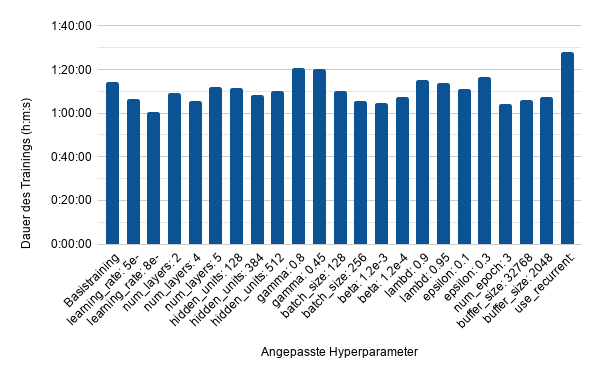
\includegraphics[scale=0.65]{images/training/training_durations.png}
\caption{Dauern der unterschiedlichen Trainingsvorgänge}
\label{fig:training_durations}
\end{figure}

Nach dem Vergleich der Ergebnisse sollte ein verlängertes, finales Training durchgeführt werden. Es wurde davon ausgegangen, dass die Parameter unabhängig voneinander verändert und schließlich kombiniert werden können, um ein optimales Ergebnis zu erzielen. Es hat sich allerdings gezeigt, dass die Nutzung mehrerer Parameteränderungen, die jeweils ein besseres Ergebnis im Vergleich zum Basistraining erzielt haben, in Kombination nicht zwangsweise ein besseres Ergebnis zur Folge haben. Damit wurde gezeigt, dass es starke Abhängigkeiten zwischen den einzelnen Parametern gibt.
In der Abbildung \ref{fig:final_training_failure} ist die entstandene Belohnungsfunktion aus diesem Training zu sehen. Es ist leicht zu erkennen, dass die Gesamtbelohnungen mit einem Maximalwert von ca. $2.6$ deutlich unter dem Niveau des Basistrainings liegen.

\begin{figure}[H]
\centering
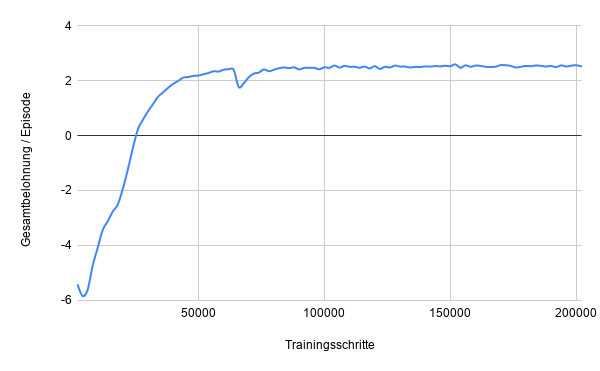
\includegraphics[scale=0.65]{images/training/final_training_failure.png}
\caption{Belohnungsfunktion durch Kombination der optimalen Einzelparameter}
\label{fig:final_training_failure}
\end{figure}

Die Ergebnisse der ausgeführten Einzeltrainings geben trotzdessen eine Auskunft über die Anpassung der Parameter im Einzelnen. Sie sind im Anhang A zu finden und werden durch Diagramme dokumentiert.

Um bei vorhandenen Abhängigkeiten zwischen den Parametern die optimalen Werte zu finden, hätte nach der Ermittlung eines neues, besseren Parameters bereits die Basiskonfiguration mit diesem Parameter angepasst werden müssen, sodass die Anpassung bei weiteren Trainingsvorgängen bereits miteinbezogen wurde.

Insgesamt stellt die Wahl der Hyperparameter ein schwieriges Problem dar, da extrem viele Kombinationen verschiedener Werte für Hyperparameter durchgeführt werden können. Einige Werkzeuge und Frameworks für Machine Learning bieten eine automatisierte Auswahl für Hyperparameter an, indem eine Menge von Kombinationen verschiedener Kandidaten für Parameter geprüft werden, um das beste Ergebnis zu erlangen. Ein Beispiel für dieses Vorgehen ist die sogenannte \Fachbegriff{Exhaustive Grid Search} \cite{scikit_gridsearch} des Frameworks \Fachbegriff{scikit-learn} \cite{scikit-learn}. Im Falle von ML-Agents gibt es so eine automatisierte Suche der Parameter nicht. Die Dauer der nötigen Trainingsvorgänge würde weiterhin deutlich zu hohe Maßstäbe annehmen.

